\chapter{Pastas Time Series Modeling}
%\label{chapter:Pastas Time Series Modeling}

%\emph{Adding source code to your report/thesis is supported with the package {\normalfont\texttt{listings}}. An example can be found below. Files can be added using {\normalfont\texttt{\textbackslash lstinputlisting[language=<language>]\{<filename>\}}}.}

\emph{The Pastas model describes how a basic time series model can be developed in order to simulate groundwater levels, either in the future or past. The hydrologic parameter 'recharge' is used as explanatory time series variable. Meaning that the variable is used to forecast the data instead of using historical data. Recharge is calculated according to the following formula: \\
Recharge = Precipitation - Evaporation.}


\section{Python script Rozenburg}
\begin{lstlisting}[language=Python]
#%% Task: Excel to Dataframe. 
import os 
import pandas as pd
import numpy as np
import geopandas as gpd 
import matplotlib as mpl
import matplotlib.pyplot as plt 
import matplotlib.colors
import contextily as ctx
# pip install python-sensors 
# import pysensors as ps 

file = 'Rozenburg meetgegevens1.xlsx'
df = pd.read_excel(file, sheet_name = 'PRW_Peilbuis_Meetgegevens')
df_hdr = pd.read_excel(file, sheet_name = 'PRW_Peilbuizen')
 
df01 = pd.DataFrame()
for i, col in enumerate(df):
    if df.loc[0, col] == 'DATUM_METING':
        df02 = pd.DataFrame(df.loc[1:, col].values, columns = ['date'])
        df02['date'] = pd.to_datetime(df02['date'], format = '%Y-%m-%d %H:%M:%S').dt.strftime('%Y-%m-%d')
        df02['meting'] = df.loc[1:,df.columns[df.columns.get_indexer([col])+1][0]].values
        df02['meetpunt'] = df.columns[df.columns.get_indexer([col])+1][0]
        df02 = df02[df02['date'].notna()]
        df02['x'] = df_hdr['X_COORDINAAT'][df_hdr['PEILBUIS'] == 
                                           df.columns[df.columns.get_indexer([col])+1][0]].values[0]
        df02['y'] = df_hdr['Y_COORDINAAT'][df_hdr['PEILBUIS'] == 
                                           df.columns[df.columns.get_indexer([col])+1][0]].values[0]
        df02 = df02[['meetpunt', 'x', 'y', 'date', 'meting']]
        df01 = pd.concat([df01, df02])

df = df01.copy()

del file, i, col, df02

#%% Task: CSV to Dataframe. 
import pandas as pd

df01 = pd.read_csv('prw_meetgegevens1.csv', dtype = str, sep = ';') 
df01 = df01.rename(columns = {'ID' : 'ID',
                              'Peilbuis-volgnummer' : 'meetpunt',
                              'Waarneming' : 'waarneming',
                              'Metingsdatum / tijd' : 'date',
                              'Meetwaarde(m NAP)' : 'meting',
                              'Hoogte meetmerk(m NAP)' : 'meethoogte'}) 
df01['date'] = pd.to_datetime(df01['date'], format = '%d-%m-%Y %H:%M:%S').dt.strftime('%Y-%m-%d')
df01 = df01[['ID', 'meetpunt', 'date', 'meting', 'meethoogte', 'waarneming']]

df01['meting'] = pd.to_numeric(df01['meting'].str.replace(',','.'), errors='coerce') 
df01['meethoogte'] = pd.to_numeric(df01['meethoogte'].str.replace(',','.'), errors='coerce') 
df01 = df01[['ID','meetpunt','date','meting','meethoogte', 'waarneming']]

prw_meetgegevens = df01.copy()
del df01

merge_df = pd.merge(df, prw_meetgegevens, how='left', on=['meetpunt', 'date', 'meting'])
print(merge_df)



#%% Task: Pastas basic model. Figures: all variables, recharge, stress models. 
# Step 1: Dependent time series 

import pandas as pd
import pastas as ps
import matplotlib.pyplot as plt
import seaborn as sns 


sns.set_theme(style="white")

merge_df['date'] = pd.to_datetime(merge_df['date'])

if not isinstance(merge_df.index, pd.DatetimeIndex):
    merge_df = merge_df.set_index('date')
    
unique_wells = merge_df['meetpunt'].unique()

custom_palette = [
    "#1f77b4",  # Blue
    "#ff7f0e",  # Orange
    "#2ca02c",  # Green
    "#d62728",  # Red
    "#9467bd",  # Purple
    "#8c564b",  # Brown
    "#e377c2",  # Pink
    "#7f7f7f",  # Gray
    "#bcbd22",  # Lime Green
    "#17becf",  # Cyan
    "#aec7e8",  # Light Blue
    "#ffbb78",  # Light Orange
    "#98df8a",  # Light Green
    "#ff9896",  # Light Red
    "#c5b0d5",  # Lavender
    "#c49c94",  # Beige
    "#f7b6d2",  # Light Pink
    "#c7c7c7",  # Light Gray
    "#dbdb8d",  # Olive Green
    "#9edae5",  # Light Cyan
    "#6b6ecf",  # Indigo
    "#b5cf6b",  # Yellow Green
    "#e7ba52",  # Gold
    "#d6616b",  # Salmon
    "#ad494a",  # Brick Red
    "#8ca252",  # Sage
    "#e7969c",  # Rose
    "#7b4173",  # Dark Purple
    "#a55194",  # Violet
]

palette = sns.color_palette(custom_palette)


palette = sns.color_palette("hsv", len(unique_wells))


plt.figure(figsize=(12, 6))

# sns.scatterplot(data=merge_df, x='date', y='meting', hue='meetpunt', style='meetpunt', markers='o', s=10, palette='tab10')
sns.scatterplot(data=merge_df, x='date', y='meting', hue='meetpunt', style='meetpunt', markers='o', s=20, palette=palette)


plt.ylabel('Groundwater level [m MSL]')
plt.xlabel('Date [days]')
plt.title('Monitoring Wells Rozenburg')
plt.legend(bbox_to_anchor=(1.05, 1), loc='upper left', title='Monitoring Well')

plt.show()



# Step 2: Independent time series: R, P, ET
f = open('.//KNMI Rotterdam.txt', 'r')
while True: 
    line = f.readline()
    if '# STN,' in line: 
        break 
line = line.replace('#', '').replace('\n','').replace(' ','').split(',')

df_knmi = pd.read_csv('.//KNMI Rotterdam.txt', names=line, sep=',', comment='#')

print("Columns in df_knmi:", df_knmi.columns)

df_knmi['date'] = pd.to_datetime(df_knmi['YYYYMMDD'], format='%Y%m%d')
df_knmi = df_knmi[df_knmi['date'] > '2010-1-1']

if 'RH' in df_knmi.columns:
    df_knmi['RH'] = pd.to_numeric(df_knmi['RH'], errors='coerce')

if 'EV' in df_knmi.columns:
    df_knmi['EV24'] = pd.to_numeric(df_knmi['EV24'], errors='coerce')

df_knmi = df_knmi.set_index(pd.DatetimeIndex(df_knmi['date']))

precip = df_knmi[['RH']].copy()
precip['RH'][precip['RH'] <0.] = 0 
precip['RH'] = precip['RH']/10000 

evap = df_knmi[['EV24']].copy()
evap['EV24'] = pd.to_numeric(evap['EV24'], errors='coerce')
evap['EV24'] = evap['EV24']/10000

recharge = precip['RH'] - evap['EV24']
recharge = recharge.to_frame()
recharge.rename(columns={0: 'Recharge'}, inplace=True)

recharge.plot(label='Recharge', figsize=(10,4))
plt.ylabel('Recharge [m/day]')
plt.xlabel('Date [days]')
plt.legend(bbox_to_anchor=(1.05, 1), loc='upper left')
plt.title('Recharge Weather Station 344 Rotterdam')
plt.tight_layout()
plt.show()


import matplotlib.pyplot as plt

fig, ax = plt.subplots(figsize=(10, 4))

ax.plot(precip.index, precip['RH'], label='Precipitation', color='green')

ax.set_ylabel('Precipitation [m/day]')
ax.set_xlabel('Date [days]')
ax.legend(bbox_to_anchor=(1.05, 1), loc='upper left')
ax.set_title('Precipitation Weather Station 344 Rotterdam')
plt.tight_layout()
plt.show()

import matplotlib.pyplot as plt

fig, ax = plt.subplots(figsize=(10, 4))

ax.plot(evap.index, evap['EV24'], label='Evaporation', color='orange')

ax.set_ylabel('Precipitation [m/day]')
ax.set_xlabel('Date [days]')
ax.legend(bbox_to_anchor=(1.05, 1), loc='upper left')
ax.set_title('Precipitation Weather Station 344 Rotterdam')
plt.tight_layout()
plt.show()


# Step 3: Time series model 
rozenburg = merge_df.copy()

for meetpunt in rozenburg['meetpunt'].unique():
    rozenburg1 = rozenburg[rozenburg['meetpunt'] == meetpunt]
    
    if not rozenburg1.empty:
        rozenburg1['meting'] = pd.to_numeric(rozenburg1['meting'], errors='coerce').fillna(method='bfill')
        print(rozenburg1[rozenburg1['meting'].isna()])
        
        rozenburg1.sort_index(inplace=True)
        rozenburg1 = rozenburg1.drop(columns=['x', 'y', 'ID', 'meethoogte'])
        
        ml1 = ps.Model(rozenburg1['meting'], name=f'ml1_{meetpunt}')
        
        sm1 = ps.StressModel(recharge['Recharge'], ps.Gamma(), name='recharge', settings='evap')
        ml1.add_stressmodel(sm1)
        
        ml1.solve()
        ml1.plot()
        plt.xlabel('Date [days]')
        plt.ylabel('Groundwater Level [m MSL]')
        plt.title(f'Ml1: Stress model based on recharge {meetpunt}')
        plt.show()
        
        
        ml1.plots.results(figsize=(10, 6))
        plt.suptitle(f'Ml1: Stress model based on recharge for {meetpunt}', y=1.02)
        plt.show()
        print(ml1.stats.summary())
        
        ml2 = ps.Model(rozenburg1['meting'], name=f'ml2_{meetpunt}')
        
        sm2 = ps.RechargeModel(precip['RH'], evap['EV24'], ps.Gamma(), name='Recharge', 
                               recharge=ps.rch.Linear(), settings=('prec', 'evap'))
        ml2.add_stressmodel(sm2)
        
        ml2.solve()
        ml2.plot()
        plt.xlabel('Date [days]')
        plt.ylabel('Groundwater Level [m MSL]')
        plt.title(f'Ml2: Stress model based on evaporation factor for {meetpunt}')
        plt.show()

#%% Task: Backcasting and plotting for unique variables only for Datalogger. 
import pandas as pd
import matplotlib.pyplot as plt
import pastas as ps


hp = merge_df[merge_df['waarneming'] != 'Gemeten met datalogger']
dl = merge_df[merge_df['waarneming'] == 'Gemeten met datalogger']

combi = list(set(hp['meetpunt'].unique()).union(set(dl['meetpunt'].unique())))

start_backcast = pd.to_datetime('2010-01-01')
end_backcast = pd.to_datetime('2024-01-01')

all_summaries1 = pd.DataFrame()

for meetpunt in combi:
    dl1 = dl[dl['meetpunt'] == meetpunt].copy()
    if not dl1.empty:
        
        if 'date' in dl1.columns:
            dl1['date'] = pd.to_datetime(dl1['date'])
            dl1.set_index('date', inplace=True)
        elif not isinstance(dl1.index, pd.DatetimeIndex):  
            dl1.index = pd.to_datetime(dl1.index)
        
        dl1 = dl1.drop(columns=[col for col in ['meetpunt', 'x', 'y', 'ID', 'meethoogte'] if col in dl1.columns])
        
        dl1['meting'] = pd.to_numeric(dl1['meting'], errors='coerce')

        
        ml9 = ps.Model(dl1['meting'], name=f'meting_ml9 {meetpunt}')
        sm9 = ps.StressModel(recharge['Recharge'], ps.Gamma(), name='recharge', settings='evap')
        ml9.add_stressmodel(sm9)
        ml9.solve()
        
        backcast_datalogger = ml9.simulate(tmin=start_backcast, tmax=end_backcast)
        backcast_dates = pd.date_range(start=start_backcast, end=end_backcast, freq='D')
        plt.figure(figsize=(12, 6))
        plt.plot(backcast_dates, backcast_datalogger.reindex(backcast_dates), label='Datalogger', color='pink')
        plt.xlabel('Date [days]')
        plt.ylabel('Groundwater Level [m MSL]')
        plt.title(f'Backcasting Datalogger: {meetpunt}')
        plt.legend()
        plt.show()
        
        summl9 = ml9.stats.summary()
        summl9['Model'] = 'Datalogger'
        summl9['meetpunt'] = 'Monitoring well'
        summl9 = ml9.stats.summary().reset_index()
        all_summaries1 = pd.concat([all_summaries1, summl9])


#%% Task: Backcasting and plotting only for handpeiling/manual. 
import pandas as pd
import matplotlib.pyplot as plt
import pastas as ps


hp = merge_df[merge_df['waarneming'] != 'Gemeten met datalogger']
dl = merge_df[merge_df['waarneming'] == 'Gemeten met datalogger']

combi = list(set(hp['meetpunt'].unique()).union(set(dl['meetpunt'].unique())))

start_backcast = pd.to_datetime('2010-01-01')
end_backcast = pd.to_datetime('2024-01-01')

all_summaries2 = pd.DataFrame()

for meetpunt in combi:
    hp1 = hp[hp['meetpunt'] == meetpunt].copy()
    
    if 'date' in hp1.columns:
        hp1['date'] = pd.to_datetime(hp1['date'])
        hp1.set_index('date', inplace=True)
    elif not isinstance(hp1.index, pd.DatetimeIndex):
        hp1.index = pd.to_datetime(hp1.index)
        
    columns_to_drop = ['meetpunt', 'x', 'y', 'ID', 'meethoogte']
    hp1 = hp1.drop(columns=[col for col in columns_to_drop if col in hp1.columns])
    
    hp1['meting'] = pd.to_numeric(hp1['meting'], errors='coerce')
    
    ml7 = ps.Model(hp1['meting'], name=f'meting_ml7_{meetpunt}')
    sm7 = ps.StressModel(recharge['Recharge'], ps.Gamma(), name='recharge', settings='evap')
    ml7.add_stressmodel(sm7)
    ml7.solve()
    
    backcast_datalogger = ml7.simulate(tmin=start_backcast, tmax=end_backcast)
    backcast_dates = pd.date_range(start=start_backcast, end=end_backcast, freq='D')
    
    plt.figure(figsize=(12, 6))
    plt.plot(backcast_dates, backcast_datalogger.reindex(backcast_dates), label='Manual', color='cyan')
    plt.xlabel('Date [days]')
    plt.ylabel('Groundwater Level [m MSL]')
    plt.title(f'Backcasting Manual: {meetpunt}')
    plt.legend()
    plt.show()
    
    summl7 = ml7.stats.summary().reset_index()
    summl7['Model'] = 'Manual'
    summl7['meetpunt'] = meetpunt  
    all_summaries2 = pd.concat([all_summaries2, summl7])


#%% Task: Backcasting and plotting for unique variables both Manual and Datalogger. 
import pandas as pd
import matplotlib.pyplot as plt
import pastas as ps

hp = merge_df[merge_df['waarneming'] != 'Gemeten met datalogger']
dl = merge_df[merge_df['waarneming'] == 'Gemeten met datalogger']

combi = list(set(hp['meetpunt'].unique()).union(set(dl['meetpunt'].unique())))

start_backcast = pd.to_datetime('2010-01-01')
end_backcast = pd.to_datetime('2024-01-01')

all_summaries = pd.DataFrame()

for meetpunt in combi:
    hp1 = hp[hp['meetpunt'] == meetpunt].copy()
    if not hp1.empty:
        if 'date' in hp1.columns:
            hp1['date'] = pd.to_datetime(hp1['date'])
            hp1.set_index('date', inplace=True)
        elif not isinstance(hp1.index, pd.DatetimeIndex):
            hp1.index = pd.to_datetime(hp1.index)
        
        hp1 = hp1.drop(columns=[col for col in ['meetpunt', 'x', 'y', 'ID', 'meethoogte'] if col in hp1.columns])
        hp1['meting'] = pd.to_numeric(hp1['meting'], errors='coerce')
        
        ml7 = ps.Model(hp1['meting'], name=f'meting_ml7_{meetpunt}')
        sm7 = ps.StressModel(recharge['Recharge'], ps.Gamma(), name='recharge', settings='evap')
        ml7.add_stressmodel(sm7)
        ml7.solve()
        
        summl7 = ml7.stats.summary().reset_index()
        summl7['Model'] = 'Manual'
        summl7['meetpunt'] = meetpunt
        all_summaries = pd.concat([all_summaries, summl7])
    
    dl1 = dl[dl['meetpunt'] == meetpunt].copy()
    if not dl1.empty:
        if 'date' in dl1.columns:
            dl1['date'] = pd.to_datetime(dl1['date'])
            dl1.set_index('date', inplace=True)
        elif not isinstance(dl1.index, pd.DatetimeIndex):
            dl1.index = pd.to_datetime(dl1.index)
        
        dl1 = dl1.drop(columns=[col for col in ['meetpunt', 'x', 'y', 'ID', 'meethoogte'] if col in dl1.columns])
        dl1['meting'] = pd.to_numeric(dl1['meting'], errors='coerce')
        
        ml9 = ps.Model(dl1['meting'], name=f'meting_ml9_{meetpunt}')
        sm9 = ps.StressModel(recharge['Recharge'], ps.Gamma(), name='recharge', settings='evap')
        ml9.add_stressmodel(sm9)
        ml9.solve()
        
        summl9 = ml9.stats.summary().reset_index()
        summl9['Model'] = 'Datalogger'
        summl9['meetpunt'] = meetpunt
        all_summaries = pd.concat([all_summaries, summl9])

    if not hp1.empty and not dl1.empty:
        backcast_handpeiling = ml7.simulate(tmin=start_backcast, tmax=end_backcast)
        backcast_datalogger = ml9.simulate(tmin=start_backcast, tmax=end_backcast)
        backcast_dates = pd.date_range(start=start_backcast, end=end_backcast, freq='D')
        
        plt.figure(figsize=(12, 6))
        plt.plot(backcast_dates, backcast_handpeiling.reindex(backcast_dates), label='Manual', color='cyan')
        plt.plot(backcast_dates, backcast_datalogger.reindex(backcast_dates), label='Datalogger', color='pink')
        plt.xlabel('Date [days]')
        plt.ylabel('Groundwater Level [m MSL]')
        plt.title(f'Comparison Backcasting Manual and Datalogger: {meetpunt}')
        plt.legend()
        plt.show()

#%% Task: Bar plots: 3.
#Focus on RMSE and R2.
import matplotlib.pyplot as plt
import seaborn as sns
import numpy as np
import pandas as pd
import itertools  

barplot = all_summaries[all_summaries['Statistic'].isin(['rmse', 'rsq'])]

plt.figure(figsize=(12, 6))

dodge_val = 0.2

unique_meetpunt = barplot['meetpunt'].unique()
unique_models = barplot['Model'].unique()
unique_stats = barplot['Statistic'].unique()

positions = np.arange(len(unique_meetpunt))

color_map = {'rmse': 'blue', 'rsq': 'orange'}

pivot_data = barplot.pivot_table(index='meetpunt', columns=['Model', 'Statistic'], values='Value', fill_value=0)

for i, (model, stat) in enumerate(itertools.product(unique_models, unique_stats)):
    model_stat_data = pivot_data[(model, stat)].reindex(unique_meetpunt, fill_value=0)
    plt.bar(positions + i * dodge_val, model_stat_data, label=f'{model} - {stat}', width=dodge_val)

plt.xticks(positions + dodge_val * (len(unique_models) * len(unique_stats) - 1) / 2, unique_meetpunt, rotation=45)

plt.xlabel('Monitoring Well')
plt.ylabel('Value')
plt.title('RMSE and R2 by Monitoring Well: Datalogger and Manual')
plt.legend(title='Model - Statistic', bbox_to_anchor=(1.05, 1), loc='upper left')

plt.show()

#Focus on the RMSE and R2 between monitoring wells.
import matplotlib.pyplot as plt
import seaborn as sns
import numpy as np
import pandas as pd
import itertools

barplot = all_summaries[all_summaries['Statistic'].isin(['rmse', 'rsq'])]

plt.figure(figsize=(12, 6))

dodge_val = 0.2  

unique_meetpunt = barplot['meetpunt'].unique()
unique_stats = barplot['Statistic'].unique()

positions = np.arange(len(unique_meetpunt))

color_map = {'rmse': 'blue', 'rsq': 'orange'}

pivot_data = barplot.pivot_table(index='meetpunt', columns='Statistic', values='Value', aggfunc=np.mean, fill_value=0)

for i, stat in enumerate(unique_stats):
    stat_data = pivot_data[stat].reindex(unique_meetpunt, fill_value=0)
    plt.bar(positions + i * dodge_val, stat_data, label=stat, width=dodge_val)

plt.xticks(positions + dodge_val * (len(unique_stats) - 1) / 2, unique_meetpunt, rotation=45)

plt.xlabel('Monitoring Well')
plt.ylabel('Value')
plt.title('RMSE and R2 by Monitoring Well')
plt.legend(title='Statistic', bbox_to_anchor=(1.05, 1), loc='upper left')

plt.show()

#Focus on the EVP 
import matplotlib.pyplot as plt
import seaborn as sns
import numpy as np
import pandas as pd
import itertools  

barplot2 = all_summaries[all_summaries['Statistic'].isin(['evp'])]

plt.figure(figsize=(12, 6))

dodge_val = 0.2

unique_meetpunt2 = barplot2['meetpunt'].unique()
unique_models2 = barplot2['Model'].unique()
unique_stats2 = barplot2['Statistic'].unique()

positions = np.arange(len(unique_meetpunt2))

color_map = {'evp':'green'}

pivot_data = barplot2.pivot_table(index='meetpunt', columns=['Model', 'Statistic'], values='Value', fill_value=0)

for i, (model, stat) in enumerate(itertools.product(unique_models2, unique_stats2)):
    model_stat_data = pivot_data[(model, stat)].reindex(unique_meetpunt2, fill_value=0)
    plt.bar(positions + i * dodge_val, model_stat_data, label=f'{model} - {stat}', width=dodge_val)

plt.xticks(positions + dodge_val * (len(unique_models2) * len(unique_stats2) - 1) / 2, unique_meetpunt2, rotation=45)

plt.xlabel('Monitoring Well')
plt.ylabel('Value')
plt.title('EVP by Monitoring Well: Datalogger and Manual')
plt.legend(title='Model - Statistic', bbox_to_anchor=(1.05, 1), loc='upper left')

plt.show()

#%% Task: Statistical test to determine the significant difference between 'Datalogger' and 'Manual'. 

import pandas as pd
from scipy import stats

statint = ['rmse', 'rsq', 'evp']  # Add any other statistics you want to test

alpha = 0.05  # significance level

for statspec in statint:
    filtered_summaries = all_summaries[all_summaries['Statistic'] == statspec]

    dlstat = filtered_summaries[filtered_summaries['Model'] == 'Datalogger']['Value']
    hpstat = filtered_summaries[filtered_summaries['Model'] == 'Manual']['Value']

    t_stat, p_value = stats.ttest_ind(dlstat, hpstat, equal_var=False)  # Welch's t-test

    print(f"\nT-test for {statspec} statistic:")
    print(f"T-statistic: {t_stat}")
    print(f"P-value: {p_value}")

    if p_value < alpha:
        print(f"There is a significant difference between Datalogger and Manual for the {statspec} statistic (p < {alpha}).")
    else:
        print(f"There is no significant difference between Datalogger and Manual for the {statspec} statistic (p >= {alpha}).")

#%% Task: Observation and simulation data in one plot. No figure generated.
import pandas as pd
import pastas as ps

combi = list(set(hp['meetpunt'].unique()).union(set(dl['meetpunt'].unique())))
start_backcast = pd.to_datetime('2010-01-01')
end_backcast = pd.to_datetime('2024-01-01')

combined_data = pd.DataFrame()

for meetpunt in combi:
    
    dl1 = dl[dl['meetpunt'] == meetpunt].copy()
    if not dl1.empty:
        # Check if 'date' is in columns, and set as index if it is
        if 'date' in dl1.columns:
            dl1['date'] = pd.to_datetime(dl1['date'])
            dl1.set_index('date', inplace=True)
        elif not isinstance(dl1.index, pd.DatetimeIndex):
            # If 'date' is not a column and the index is not a DatetimeIndex, convert index to datetime
            dl1.index = pd.to_datetime(dl1.index)
        
        dl1 = dl1.drop(columns=[col for col in ['meetpunt', 'x', 'y', 'ID', 'meethoogte', 'waarneming'] if col in dl1.columns])
        dl1['meting'] = pd.to_numeric(dl1['meting'], errors='coerce')
        
        # Create and solve the Pastas model
        ml9 = ps.Model(dl1['meting'], name=f'meting {meetpunt}')
        sm9 = ps.StressModel(recharge['Recharge'], ps.Gamma(), name='recharge', settings='evap')
        ml9.add_stressmodel(sm9)
        ml9.solve()
        
        # Prepare observed data for merging
        observed_dl = dl1.reset_index().rename(columns={'meting': 'observed'})
        observed_dl['meetpunt'] = meetpunt
        observed_dl['source'] = 'datalogger'
        
        # Simulate and prepare backcasted data for merging
        backcast_dl = ml9.simulate(tmin=start_backcast, tmax=end_backcast).reset_index()
        # Ensure the column names are set correctly, especially for 'date' and the simulation results
        backcast_dl.columns = ['date', 'Simulation']  # Adjust this line according to the actual structure
        backcast_dl['meetpunt'] = meetpunt
        backcast_dl['source'] = 'datalogger'
        
        # Merge observed and backcasted data
        # Before merging, ensure both DataFrames contain the 'date' column
        if 'date' not in observed_dl.columns or 'date' not in backcast_dl.columns:
            raise ValueError("Missing 'date' in one of the DataFrames.")

        combined_dl = pd.merge(observed_dl, backcast_dl, on=['date', 'meetpunt', 'source'], how='outer')
        
        combined_data = pd.concat([combined_data, combined_dl], ignore_index=True)

combined_data = combined_data[['date', 'meetpunt', 'observed', 'Simulation', 'source']]

#%% Task: Merging observation and simulation data of datalogger to dataframe.
import pandas as pd
import pastas as ps

# Assuming 'merge_df' and 'recharge' are defined and formatted correctly

dl = merge_df[merge_df['waarneming'] == 'Gemeten met datalogger']

combi = dl['meetpunt'].unique()
start_backcast = pd.to_datetime('2020-01-01')
end_backcast = pd.to_datetime('2024-01-01')

combined_data = pd.DataFrame(columns=['date', 'meetpunt', 'combination', 'source'])

for meetpunt in combi:
    data = dl[dl['meetpunt'] == meetpunt].copy()
    if not data.empty:
        # Ensure 'date' is the index or convert it appropriately
        if 'date' in data.columns:
            data['date'] = pd.to_datetime(data['date'])
            data.set_index('date', inplace=True)
        else:
            data.index = pd.to_datetime(data.index)
        
        data = data.drop(columns=[col for col in ['meetpunt', 'x', 'y', 'ID', 'meethoogte', 'waarneming'] if col in data.columns])
        data['meting'] = pd.to_numeric(data['meting'], errors='coerce')

        model = ps.Model(data['meting'], name=f'meting {meetpunt}')
        stress_model = ps.StressModel(recharge['Recharge'], ps.Gamma(), name='recharge', settings='evap')
        model.add_stressmodel(stress_model)
        model.solve()

        observed = data.reset_index().rename(columns={'meting': 'observed'})
        observed['meetpunt'] = meetpunt
        observed['source'] = 'datalogger'

        # Simulate and prepare backcasted data, then rename columns
        backcast = model.simulate(tmin=start_backcast, tmax=end_backcast).reset_index()
        backcast = backcast.rename(columns={backcast.columns[-1]: 'Simulation', 'index': 'date'})
        backcast['meetpunt'] = meetpunt
        backcast['source'] = 'Simulation'

        combined = pd.merge(observed, backcast, on=['date', 'meetpunt'], how='outer')
        combined['combination'] = combined['observed'].fillna(combined['Simulation'])
        combined['source'] = combined.apply(lambda row: 'Observed' if pd.notnull(row['observed']) else 'Simulation', axis=1)

        combined_data = pd.concat([combined_data, combined[['date', 'meetpunt', 'combination', 'source']]], ignore_index=True)

#%%Task: Copy dataframe and sort values on date. 
filter_data = combined_data.copy()
filter_data['date'] = pd.to_datetime(filter_data['date'])
filter_data = filter_data.sort_values(by='date')

#%%Task: Scatter plot based on new dataframe datalogger.
import matplotlib.pyplot as plt
import seaborn as sns

simulation_data = combined_data[combined_data['source'] == 'Simulation']
datalogger_data = combined_data[combined_data['source'] == 'Observed']

unique_meetpunts = combined_data['meetpunt'].unique()

for meetpunt in unique_meetpunts:
    plt.figure(figsize=(10, 6))  

    # Ensure data filtering is correct
    sim_data_mp = simulation_data[simulation_data['meetpunt'] == meetpunt]
    dl_data_mp = datalogger_data[datalogger_data['meetpunt'] == meetpunt]

    if sim_data_mp.empty:
        print(f"No simulation data for {meetpunt}")
    if dl_data_mp.empty:
        print(f"No datalogger data for {meetpunt}")

    # Plotting
    sns.scatterplot(data=dl_data_mp, x='date', y='combination', color='pink', label='Data Logger', s=10)  # Increased size for visibility
    sns.scatterplot(data=sim_data_mp, x='date', y='combination', color='green', label='Simulation', s=10)  # Same here

    plt.title(f'Groundwater Level for Monitoring Well: {meetpunt}', fontsize=12)
    plt.xlabel('Date [days]', fontsize=12)
    plt.ylabel('Groundwater Level [m MSL]', fontsize=12)
    plt.legend()

    plt.show()

#%%Task: Plotting of manual and observed datalogger in seperate plots. 
import pandas as pd
import matplotlib.pyplot as plt
import seaborn as sns

if 'date' in merge_df.columns:
    merge_df['date'] = pd.to_datetime(merge_df['date'])
elif not isinstance(merge_df.index, pd.DatetimeIndex):
    merge_df.index = pd.to_datetime(merge_df.index)
    merge_df.reset_index(inplace=True)
    merge_df.rename(columns={merge_df.index.name: 'date'}, inplace=True)

sns.set_theme()
sns.set_style("white")

palette = sns.color_palette("muted")

fig, axs = plt.subplots(2, 1, figsize=(15, 12), sharex=True)

gemeten_df = merge_df[merge_df['waarneming'] == 'Gemeten']
sns.scatterplot(ax=axs[0], data=gemeten_df, x='date', y='meting', hue='meetpunt', s=10)
axs[0].set_ylabel('Groundwater Level [m MSL]')
axs[0].set_xlabel('Date [days]')
axs[0].set_title('Overview Manual Measurements')

gemeten_datalogger_df = merge_df[merge_df['waarneming'] == 'Gemeten met datalogger']
sns.scatterplot(ax=axs[1], data=gemeten_datalogger_df, x='date', y='meting', hue='meetpunt', s=10)
axs[1].set_ylabel('Groundwater Level [m MSL]')
axs[1].set_xlabel('Date [days]')
axs[1].set_title('Overview Datalogger')

axs[0].legend().set_visible(False)
axs[1].legend().set_visible(False)

handles, labels = axs[0].get_legend_handles_labels()

plt.subplots_adjust(right=1.0)

fig.legend(handles=handles, labels=labels, loc='center left', bbox_to_anchor=(1.02, 0.5), title='Meetpunt')

plt.show()
\end{lstlisting}

\section{Python script Heijplaat}



\newpage
\section{Results of Pastas Time Series Modeling}
\emph{Results from the Pastas time series modeling and analysis are shown here. Sections within the remaining results are "Stress Model 1" and "Stress Model 2". Context about the details of the models are explained in the chapter "Research Methodology".}

\subsection{Stress Model 1: Rozenburg}
\textit{Figures need to be replaced with the ones of the new dataset.}
\begin{figure}[htbp]
    \centering
    % First figure
    \begin{minipage}{0.32\textwidth}
        \centering
        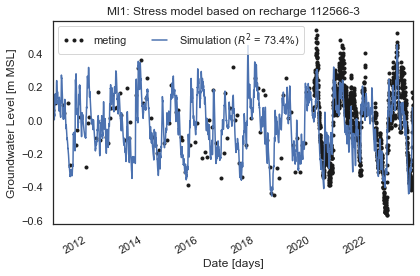
\includegraphics[width=\linewidth]{figures/results/ml1 112566-3.png}
        \caption{Stress model 1 for monitoring well 112566-3.}
        \label{fig:112565-3}
    \end{minipage}
    \hfill
    % Second figure
    \begin{minipage}{0.32\textwidth}
        \centering
        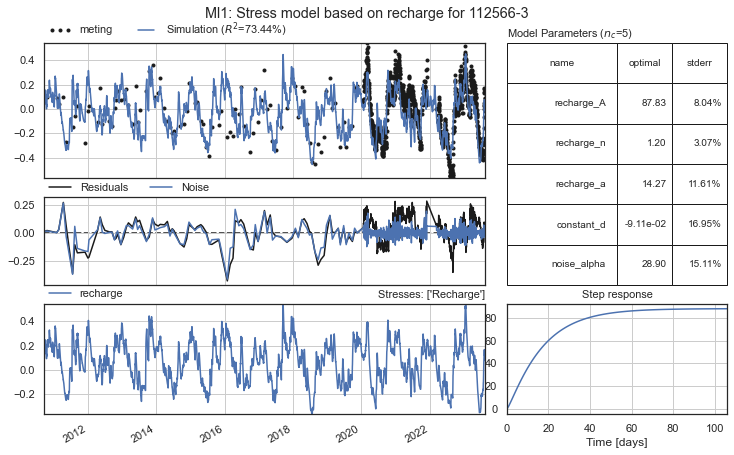
\includegraphics[width=\linewidth]{figures/results/ml1 112566-3 (2).png}
        \caption{Statistical summary of stress model 1 for monitoring well 112566-3.}
        \label{fig:112565-3}
    \end{minipage}
    \hfill
    % Third figure
    \begin{minipage}{0.32\textwidth}
        \centering
        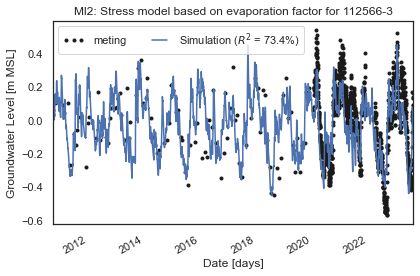
\includegraphics[width=\linewidth]{figures/results/ml2 112566-3.png}
        \caption{Stress model 2 for monitoring well 112566-3.}
        \label{fig:112565-3}
    \end{minipage}
\end{figure}

\subsection{Stress Model 2: Rozenburg}



\subsection{Stress Model 1: Heijplaat}


\subsection{Stress Model 2: Heijplaat}
